\documentclass[12pt]{article}
\usepackage{graphicx}
\usepackage{float}
\usepackage{amsmath}
\setlength{\parskip}{5mm}
\renewcommand{\baselinestretch}{1.0}

\title{Project Report 2 : 3D Shape Search Engine}
\author{Brian R. Cairl}
\begin{document}
\maketitle
\pagebreak

\newcommand{\ith}{i$^{th}$\hspace{0.5mm}}
\newcommand{\jth}{j$^{th}$\hspace{0.5mm}}
\newcommand{\kth}{j$^{th}$\hspace{0.5mm}}
\newcommand{\st}{\hspace{0.5mm}:\hspace{0.5mm}}
\newcommand{\fa}{\hspace{0.5mm}\forall\hspace{0.5mm}}


\section*{Introduction}

	\noindent	
	This report details the design and testing of a 3D shape search engine which leverages several types of 3D shape descriptors. In particular, this search engine makes use of Geodesic distance (GD) and Euclidean distance (ED) shape descriptors (as well as a custom, curvature-base descriptor) to generate a pairwise similarity measures (a \emph{distance}) between 3D meshes. The contents of this report will include a description of the code written to generate both GD and ED descriptors, given a 3D shape (mesh) input; a description of how noise and distortion were added to a set of 3D models (TOSCA data set); a description of how the search-engine was implemented, and a corresponding GUI front-end for 3D shape retrieval; and an experimental comparison between GD and ED based searches when clean, distorted and incomplete models are presented to the aforementioned search engine. Additionally, a tutorial will be provided as to how to run the search-engine GUI.

	\noindent	
	In addition to aforementioned project requirements, this report will also present the result of a custom feature descriptor when applied to 3D shape matching. This custom descriptor, dubbed the \emph{CD}, or curvature-dissimilarity descriptor, utilizes pair-wise dot products of unit normals which emanate from the triangular faces of each mesh. The formulation of this descriptor will be covered in detail at the end of this report, and will be compared to the performance of the GD and ED descriptors when applied to shape searching.


\section*{GD and ED Descriptors}
	
	\noindent
	Geodesic-distance (GD) and Euclidean Distance (ED) descriptors are histogram-based 3D descriptors used in the identification of 3D shapes. These descriptors are utilized to represent a 3D shape as high-dimensional feature vector. This section will describe the MATLAB implementation of a GD/ED descriptor generator used throughout this project.

	\noindent
	 GD and ED descriptors are generated using the MATLAB functions \emph{create\_GDdescriptor} and \emph{create\_EDdescriptor}, respectively. Each function takes a single mesh-structure argument, by default. The mesh structure contains two member variables which contain a list of vertices, $V$, and edge connections, $E$, respectively. Within each of these functions, corresponding GD and ED values are calculated between some percentage of the vertices (to all other vertices) within each mesh and binned using a function  \emph{bin\_values(d,dmin,dmax,dres)}, which creates a histogram (feature vector) from a vector of distances, $d$. Here we consider only a percentage of the mesh during feature-vector generation for the sake of saving computation time. The generated histogram has a minimum and maximum binning distance of $dmin$ and $dmax$; and a binning resolution of $dres$. Henceforth, distance values are counted into the \jth bin of each \ith histogram, $h_{j}^{i}$, as follows:
	\begin{equation}
    		h_{j}^{i} = 
		\sum_{d \in D}  
		\begin{cases}
    		1,	& (\text{dmin} + \text{dres}*j) < d < (\text{dmin} + \text{dres}*(j+1))  \\
    		0,   & \text{otherwise}
		\end{cases}
	\end{equation}
	To clarify, each histogram,  $H^{i} = [h_{1}^{i},h_{2}^{i},...,h_{N}^{i}]$, is created using distances from the \ith vertex to \emph{all} other vertices in the provided mesh. Once histograms generated for each sample vertex, they are summed (in an element wise fashion) and then normalized by the number of sample vertexes considered in feature generation. We can, therefore, write the final feature vector, $x\in\Re^{N}$, by:
%%
	\begin{equation}
		x = \frac{1}{n_{\text{vectices}}}\sum_{i} H^{i}
	\end{equation}
	The dimensionality of $x$, $N$, is determined by :
	\begin{equation}
		N = \text{ceil}\left( \frac{\text{dmax} - \text{dmin} }{\text{dres}} \right)
	\end{equation}
%%
	\noindent
	In descriptor generation, $1\%$ of the vertices of each mesh were considered during distance calculation. Histogram parameters have been chosen as follows:
	\begin{itemize}
	\item{$dmin = 0$}
	\item{$dmin = 600$}
	\item{$dres = 1$}
	\end{itemize}

	\noindent
	As for the distance calculations, separate GD and ED functions have been written to handle the calculation of distance between a sample vertex and all other vertices in a mesh. To calculate the GD between points, a shortest path algorithm, $dijkstras(G,i)$ has been written which calculates the shortest  distance between a node, $i$, to all other nodes in a graph $G$, as well as the associated pathing information. The graph $G$ is represented as an adjacency matrix whose edge connections are computed as euclidean distances between connected nodes. The graph $G$ is generated from an input mesh $M$ by a separate function \emph{mesh2graph(M,p)} which converts the mesh structure to the aforementioned adjacency-matrix structure. The input parameter $p$ is used to set the order of the $L_{p}$-norm distance to be computed between each graph node. To compute the euclidean distance between points, $p$ is, obviously, set to $p=2$.
	
	\noindent
	To calculate the ED between points, an $L_{2}$ norm calculation performed on the vector difference between each \ith sample vertex and all other vertices of the mesh $M$. This calculation is performed from within the driver function, \emph{create\_EDdescriptor}, a helper subroutine, \emph{euclidean}.


\section*{Proposed CD Descriptor}

	\noindent
	Along with the standard GD and ED descriptors, a proposed descriptor is tested for search engine use which considers curvature relationships between pairs of mesh faces. The MATLAB function  \emph{create\_CDdescriptor} is used to create such a descriptor. The CD descriptor is also a histogram-based shape descriptor which is built upon the angular dissimilarities between pairs of mess faces. To compute this descriptor, a centroid and unit normal corresponding to each mesh face are computed to represent said face as a planar geometry. The computation of each \ith point-normal $p_{i} = [ c_{i}^T, \vec{u}_{i}^T ] \in \Re^{6\times1}$ is carried out as follows:

	\begin{equation}
		c_{i} = \frac{1}{3}\sum_{j=1}^{3} v_{e_{j}}
	\end{equation}
	\begin{equation}
		\vec{u}_{i} = \frac{( v_{e_{1}} - v_{e_{2}}) \times ( v_{e_{3}} - v_{e_{2}})}{|( v_{e_{1}} - v_{e_{2}}) \times ( v_{e_{3}} - v_{e_{2}})|}
	\end{equation}
	where $e=[e_{1},e_{2},e_{3}]$ is a triad of indices used to select which vertices belong to each triangular face, and $v\in\Re^{3}$ are the vertices of the source mesh.

	\noindent
	Once all point-normal representations of each face have been computed, the normal component of each \ith face is stacked into a matrix $U = [u_{1},u_{2},...,u_{m}]\in\Re^{3\times m}$. The curvature relationship between all faces is then obtained by $C = (U^T U) \in \Re^{m \times m}$, where each \kth row of $C$ contains the $\cos(*)$ of the angular difference between the normal of each \kth face and all other faces. These differences are then binned into histograms, much like in the formulations for the GD and ED descriptors. Binning parameters for this descriptor class are as follows:
	\begin{itemize}
	\item{$dmin = -1$}
	\item{$dmin = 1$}
	\item{$dres = 0.001$}
	\end{itemize}


	\subsection*{Distance measure for shape matching}

		\noindent
		During shape-matching process, the distance (scalar dissimilarity) between shapes is determined by the distance between associated feature vectors. For a pair of meshes $A$ and $B$ with associated feature vectors $x^{A}$ and $x^{B}$, shape dissimilarity, $d_{AB}$ is calculated by:

		\begin{equation}
			d_{AB} = \sqrt{ \sum_{i=0}^{N-1} \left( x^{A}_{i} - x^{B}_{i} \right)^{2} }
			\label{eq::shape_distance}
		\end{equation} 



\section*{Noise and Mesh Distortion simulation}
	
	\noindent
	For the purpose of testing the robustness of the ED and GD descriptors, and in-turn the 3D shape search-engine, the provided (reduced) TOSCA dataset is augmented with noisy and incomplete versions of the original clean models.

	\subsection*{Noisy Datasets}

		\noindent
		Noisy models are generated by adding Gaussian noise to each clean model in the original database. Each original mesh is modified using the provided function \emph{addGaussianNoise} for three levels of Gaussian noise. Therefore, three (low, med, high) noisy data models are generated for each clean model. Noise levels are chosen to be 0.001, 0.008 and 0.015 for the low, medium and high noise models respectively. Noisy mesh generation is automated with a script named \emph{noisy\_query\_set\_generation}, which generates new noisy models from each original, clean model for each level of noise. Figure \ref{fig::veryNoisyCat} shows a comparison between a clean and noisy model.

	\begin{figure}[!h]
		\centering
		\fbox{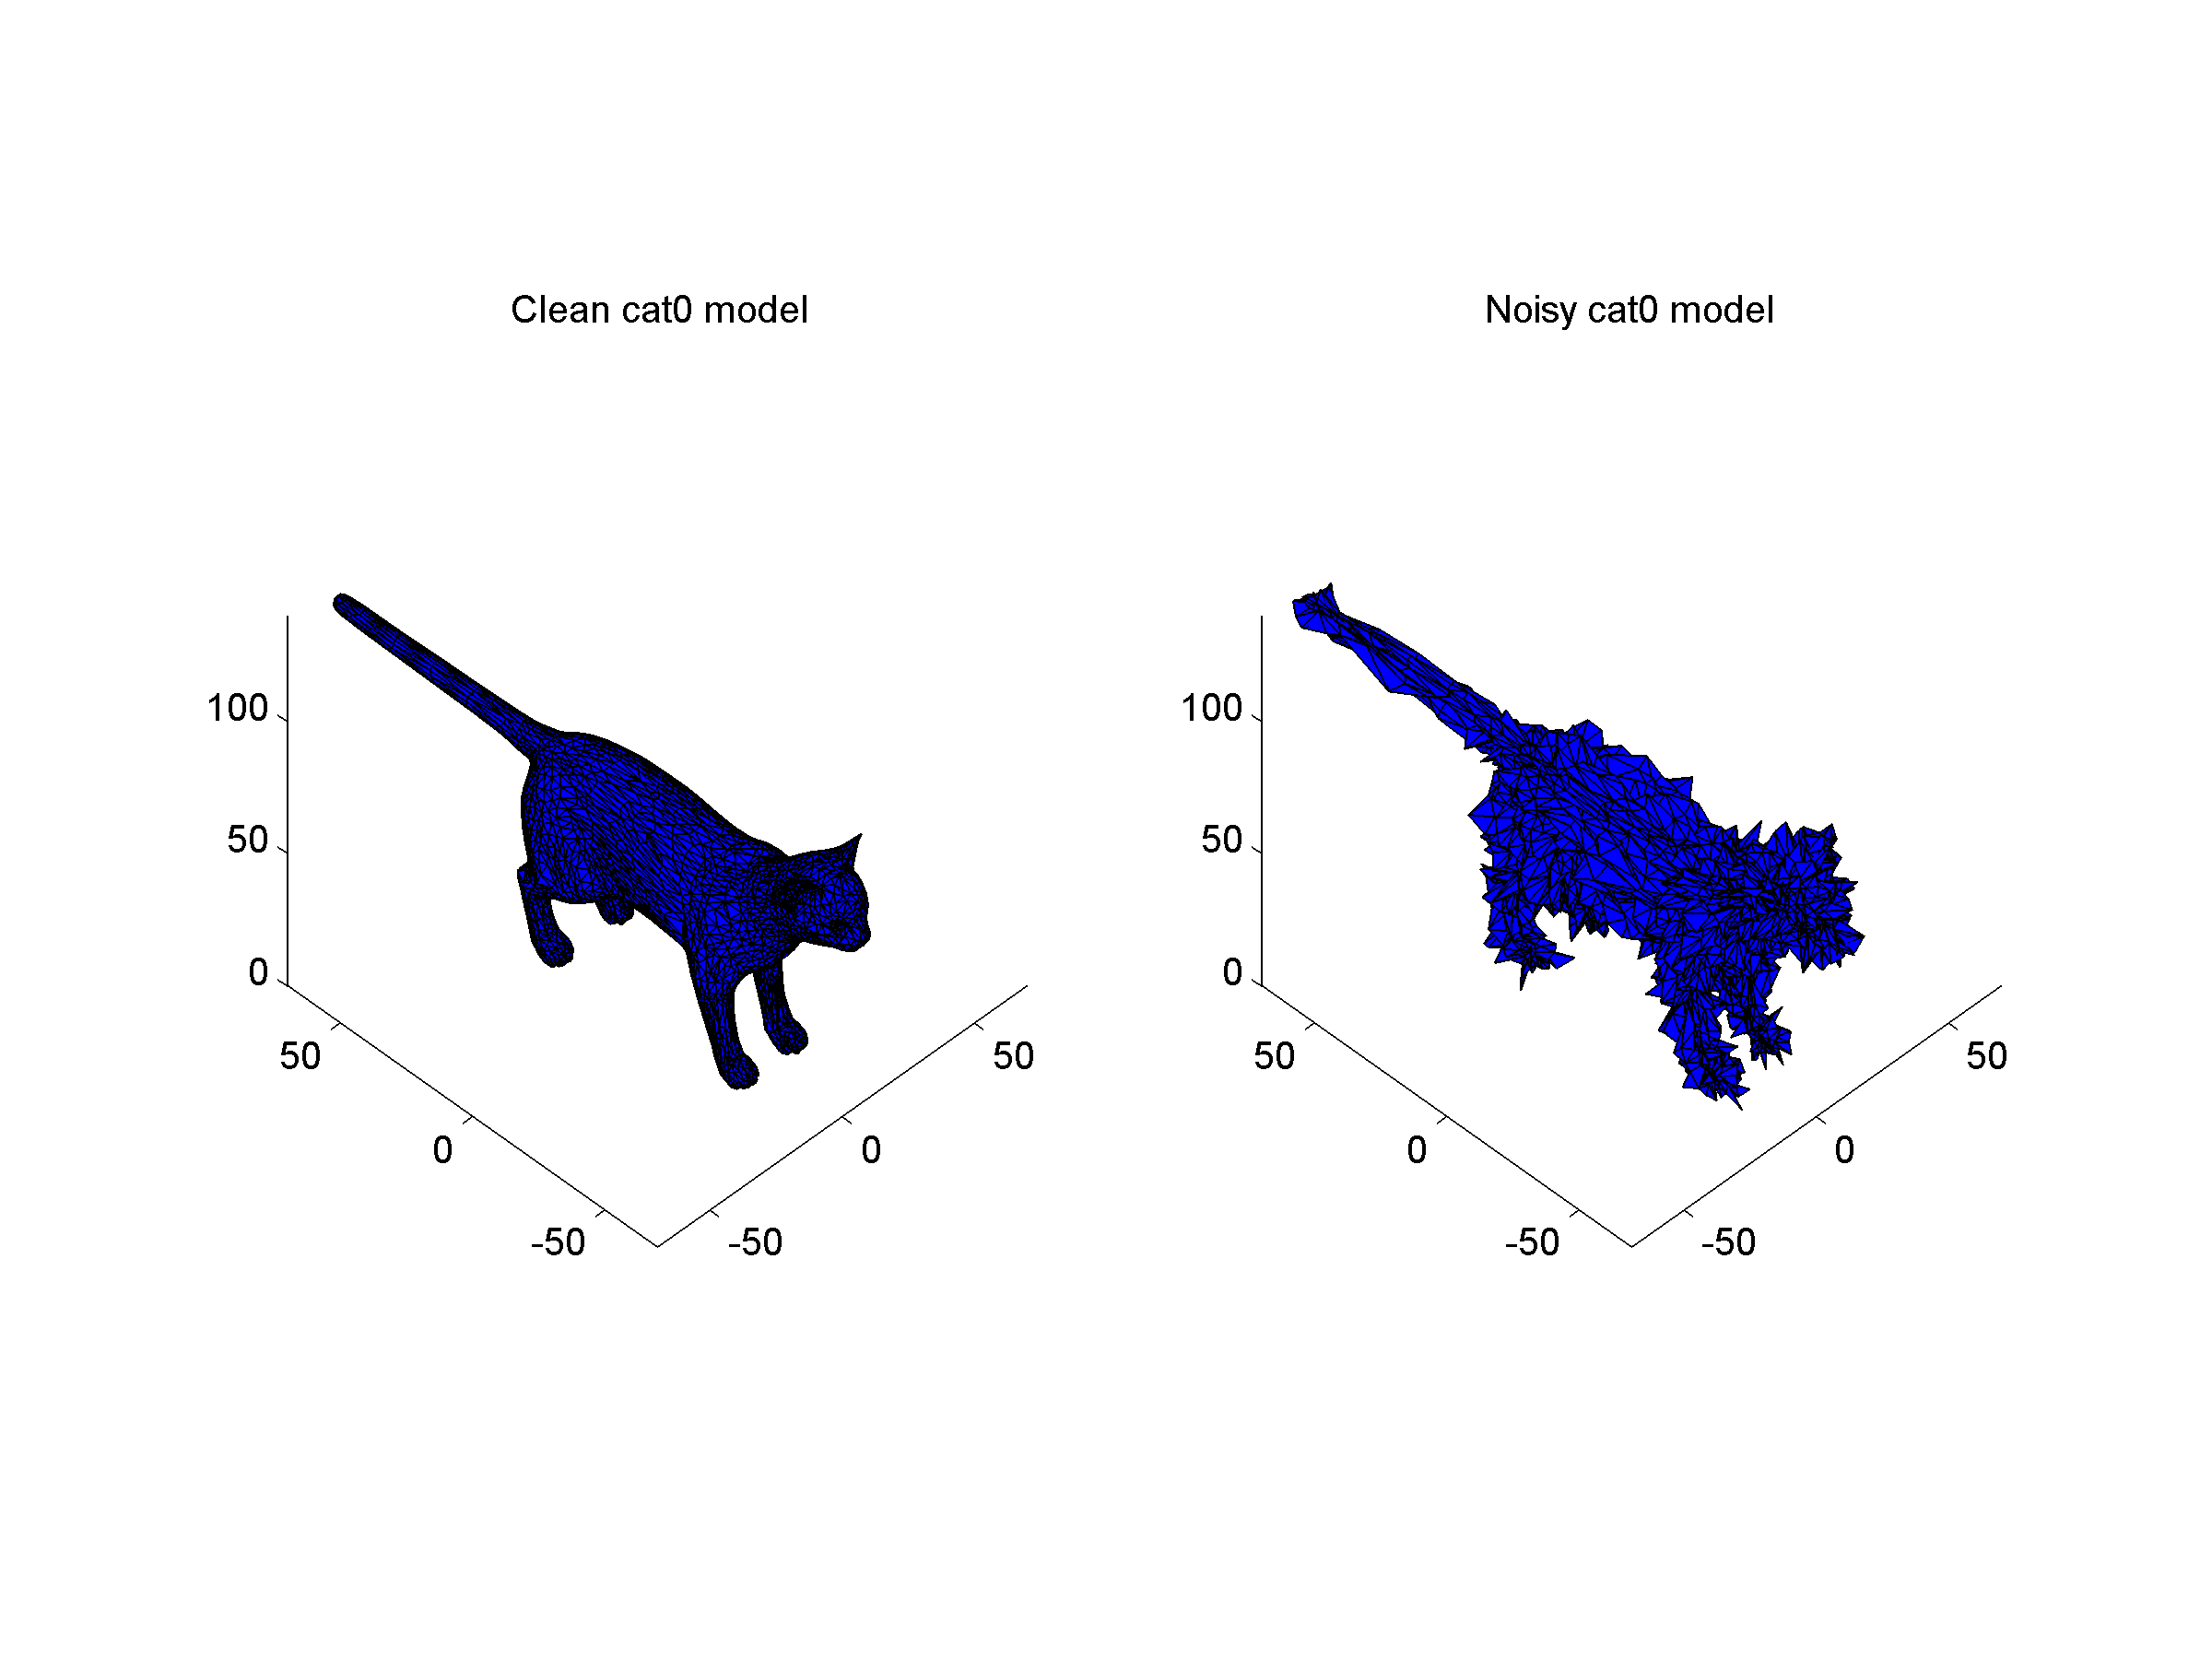
\includegraphics[width=\textwidth]{plots/noisy_clean.png}}
		\caption{Comparison of a clean and noisy model}
		\label{fig::veryNoisyCat}
	\end{figure}


	\subsection*{Incomplete Datasets}

		\noindent
		Three incomplete models are generated for each clean model by removing incrementally larger portions of each original mesh using the program MeshLab. Namely, low, medium, and highly effected models are generated by the aforementioned process. Any resulting holes in the effect mesh are filled using an hole-filling algorithm built into the MeshLab software. Figure \ref{fig::veryDeadCat} shows a comparison between a clean and incomplete model.
 
	\begin{figure}[!h]
		\centering
		\fbox{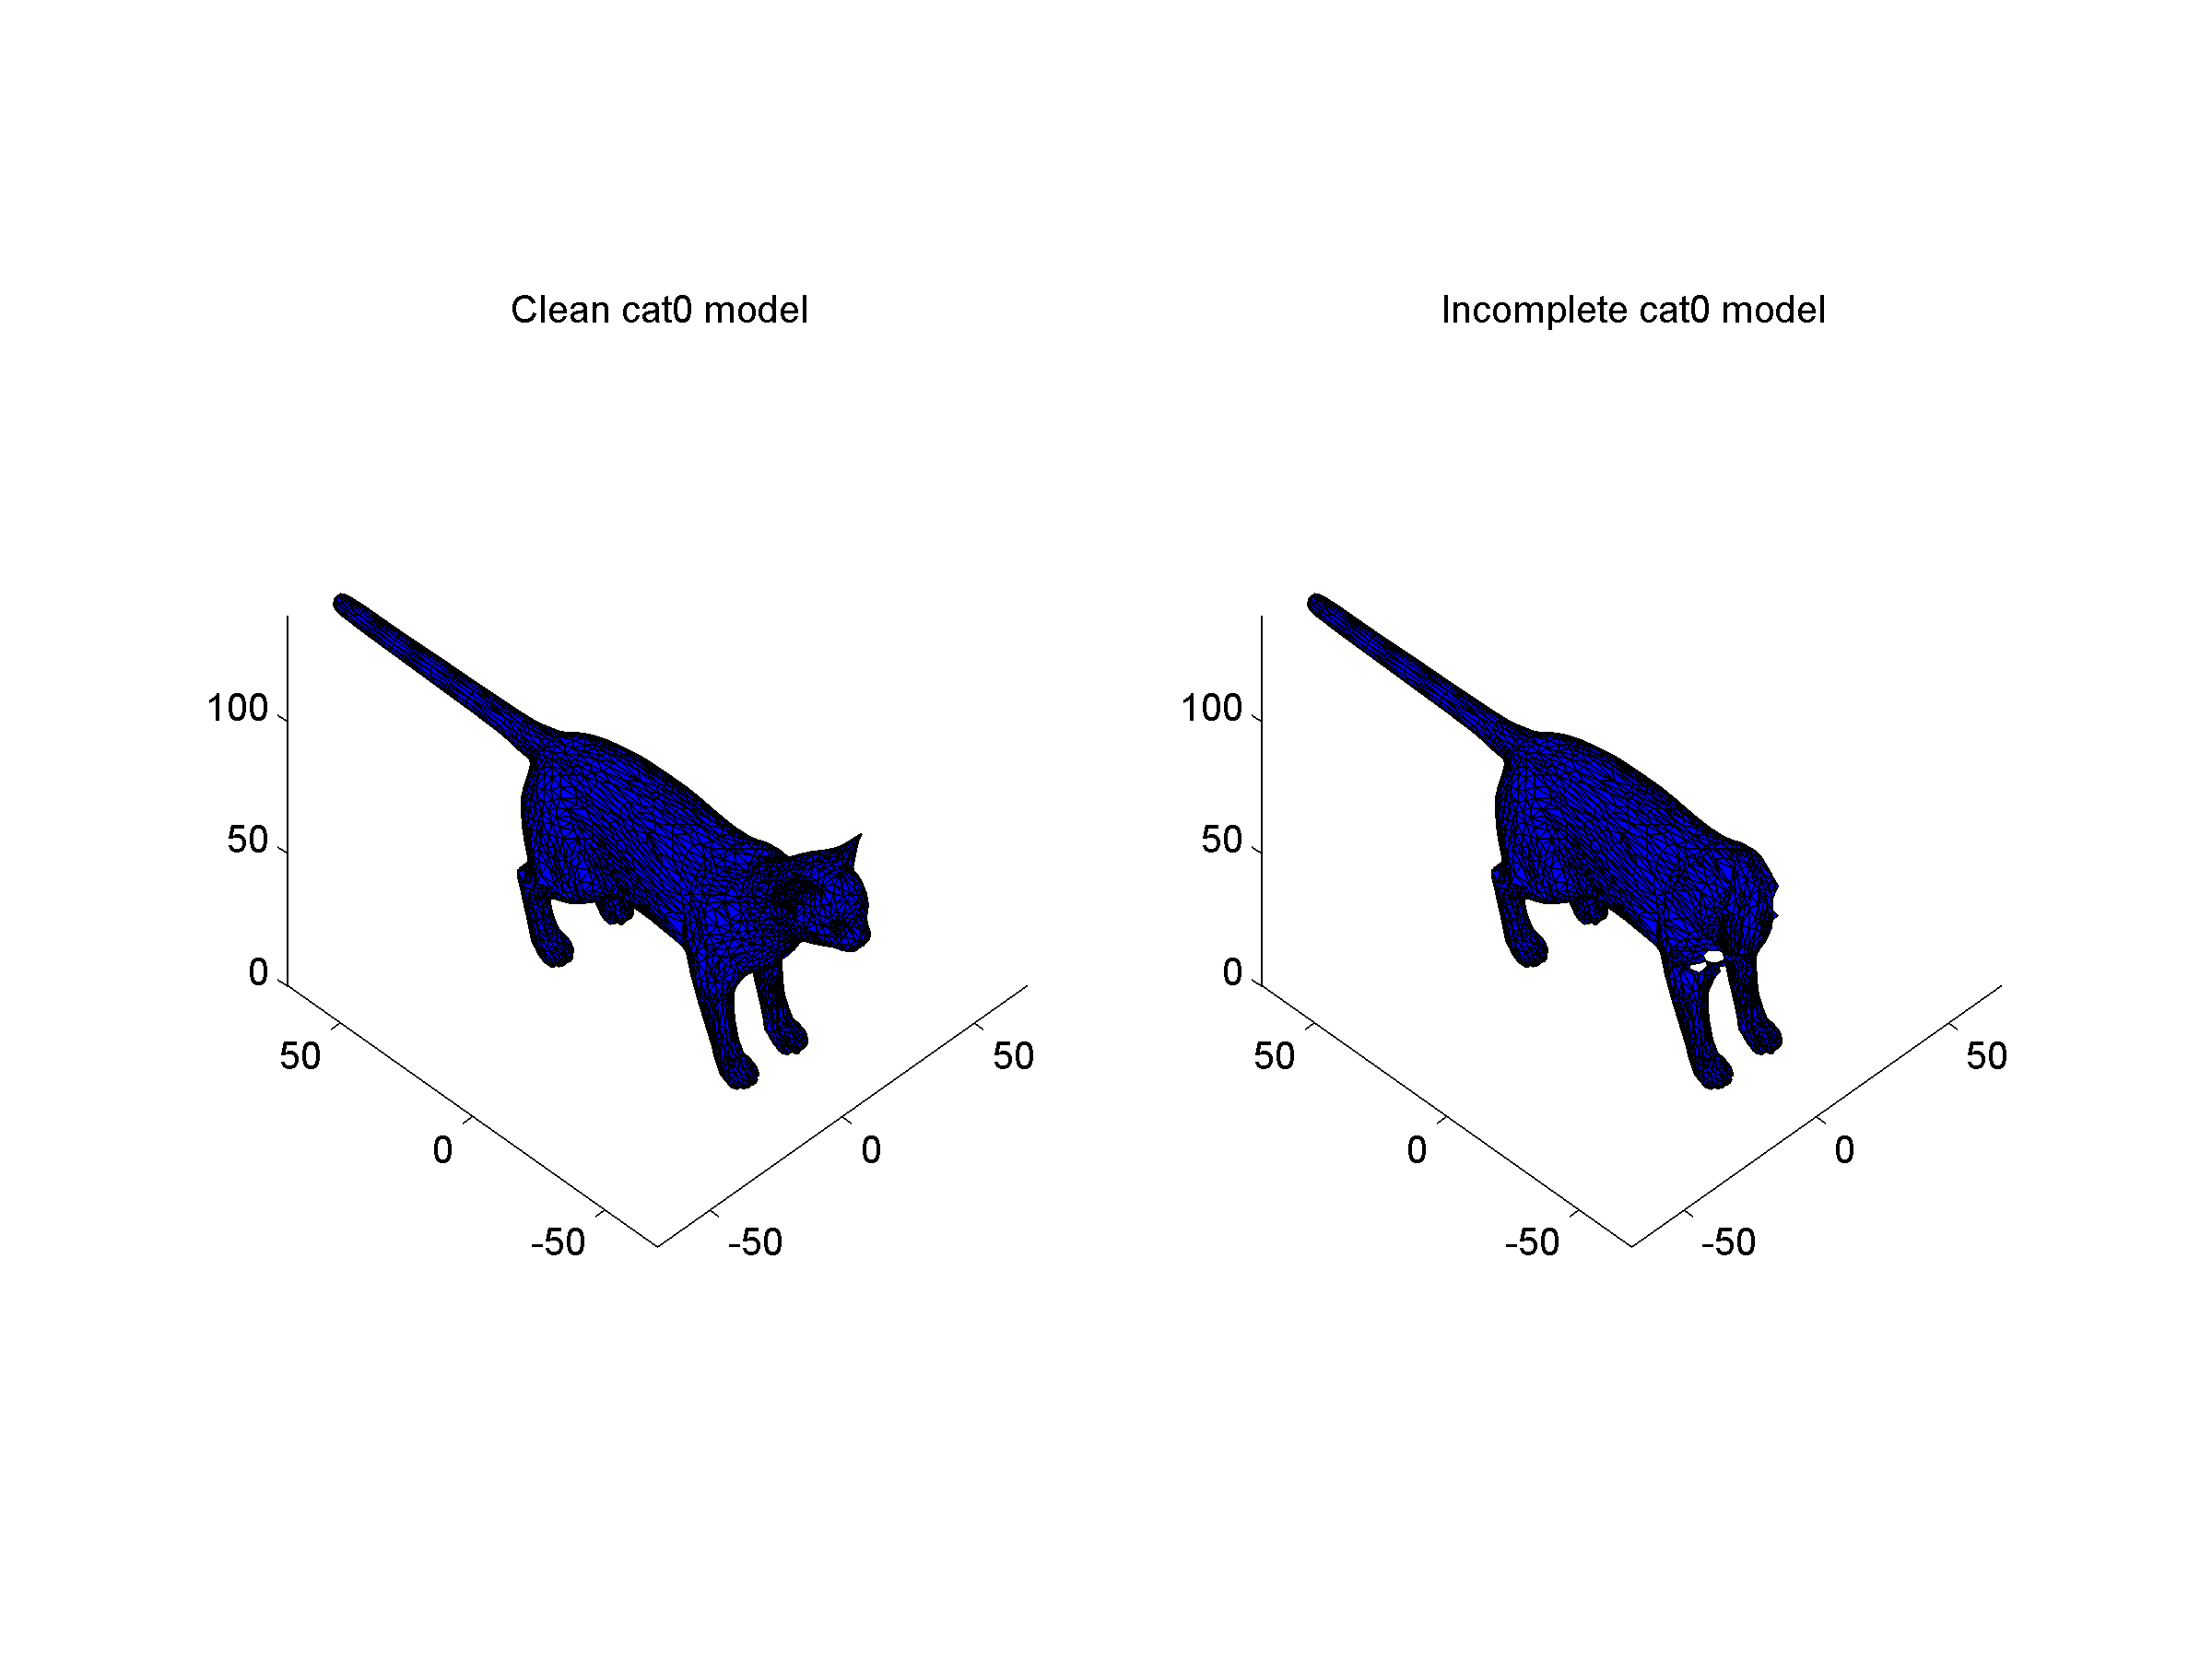
\includegraphics[width=\textwidth]{plots/incomp_clean.png}}
		\caption{Comparison of a clean and noisy model}
		\label{fig::veryDeadCat}
	\end{figure}


\section*{The 3D Shape Search Engine (and GUI)}

	\noindent
	The 3D search engine, implemented as a MATLAB function \emph{search\_engine}, creates a ranked list of models (from closest to furtherest) from a query model (referenced by name). The function takes string arguments for a query model name; the name of a folder which contains a database of \emph{metamesh} information files; and a descriptor type to use for matching. For the sake of speed, all model/query meshes have been pre-processed as \emph{metamesh} objects. These objects have been coded as a separate MATLAB \emph{classdef} with several convenience functions. The \emph{metamesh} class contains a mesh member variable, which contains the original mesh data; three descriptor member variables for each of the GD, ED, and CD descriptors, respectively; and strings which correspond to the mesh's source-file path, name and class information. A function \emph{metamesh.dist} is used to compute the relative distance between a pair of \emph{metamesh} objects with respect to all three descriptors. Additional functions for displaying the source mesh have been added which call a helper function \emph{meshview}, which acts as a simplified wrapper for the MATLAB built-in function \emph{patch}.

	\noindent
	When run, the search engine functions computes the pair-wise distances between a query \emph{metamesh} and all \emph{metamesh} files in the specified database folder. The engine returns an $N\times2$ cell of \emph{metamesh} objects, ordered from closest to furthest from the specified query model. \emph{metamesh} files are generated from an original set of query meshes (clean, noisy and incomplete) using a script, \emph{generate\_meta\_meshes}, which automates the conversion process.


	\subsection*{How to run the Search Engine GUI}

	\noindent
	The search-engine GUI is contained in the files \emph{model\_search.m}, which contains all GUI callbacks; and \emph{model\_search.fig}, which describes the GUI layout. To run the GUI on a particular model search, the name of a model is entered into a text-input box (red) located on the ``User Controls" panel, and a particular descriptor to search on is selected from a drop-down list (green), as shown in Figure \ref{fig::tut0}.
	
	\begin{figure}[!h]
		\centering
		\fbox{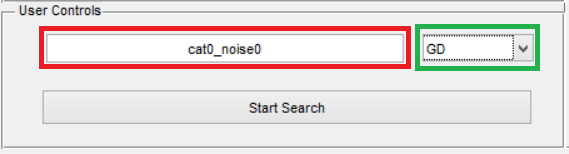
\includegraphics[width=\textwidth]{tutorial/select.png}}
		\caption{Model input and descriptor selection}
		\label{fig::tut0}
	\end{figure}

	\noindent
	After the aforementioned parameters have been set, a search is performed by hitting the ``Start Search" button (orange), as shown in Figure \ref{fig::tut1}.

	\begin{figure}[!h]
		\centering
		\fbox{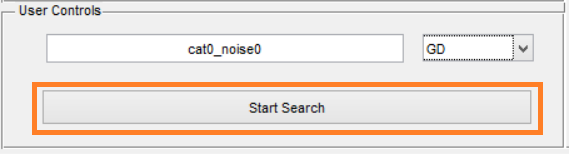
\includegraphics[width=\textwidth]{tutorial/search.png}}
		\caption{Starting the model search}
		\label{fig::tut1}
	\end{figure}

	\noindent
	When the search is complete, the central ``Match" panel of the GUI shows a 3D view of the query model (blue) and the top match result (green) overlayed, as shown in Figure \ref{fig::tut2}. Below the 3D view is a plot of the histograms (overlayed) of the top-5 search results, corresponding to the results shown in the right-most panel labeled ``Top-5 Returns". The ``Top-5" panel displays the Top-5 search results, from closest to furthest going from top to bottom, for the given search. The name of each returned result, as well as its distance from the query model is shown to the right of each 3D view.
	%%
	%%
	\begin{figure}[!h]
		\centering
		\fbox{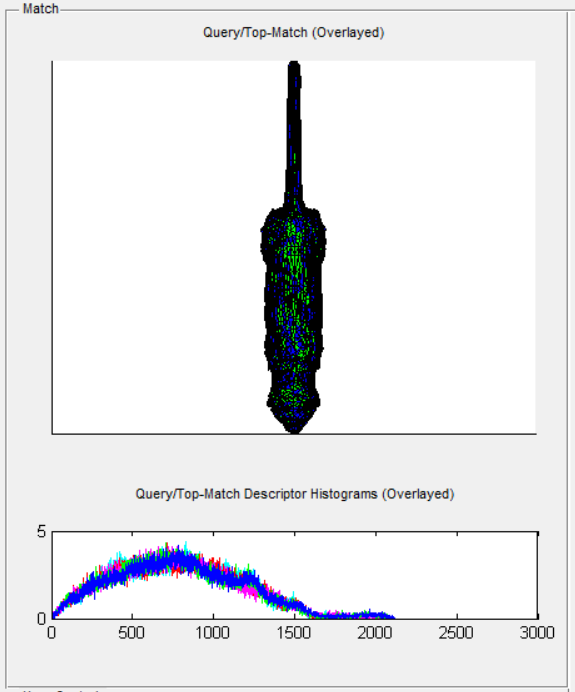
\includegraphics[scale=0.75]{tutorial/match.png}}
		\caption{Top search results}
		\label{fig::tut2}
	\end{figure}
	%%
	%%
	\noindent
	The full GUI (after a complete search) is shown in Figure \ref{fig::tut3}
	\begin{figure}[!h]
		\centering
		\fbox{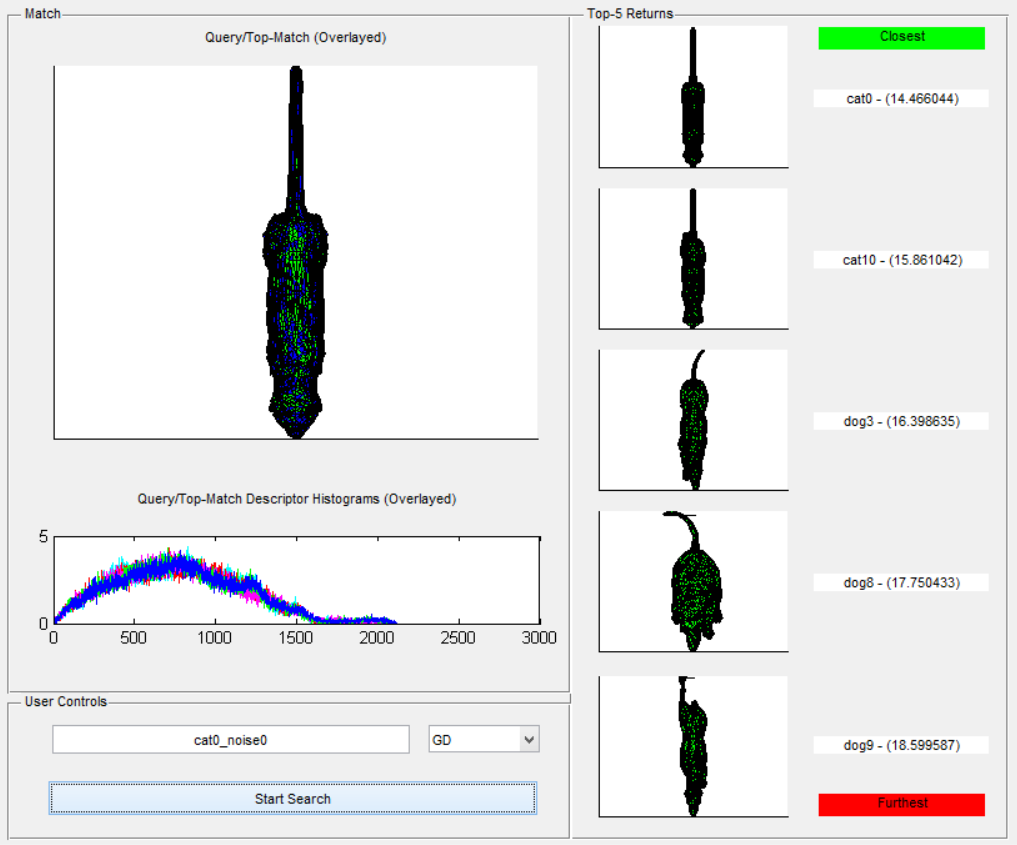
\includegraphics[scale=0.75]{tutorial/full.png}}
		\caption{Full 3D search engine GUI}
		\label{fig::tut3}
	\end{figure}

\section*{Search Engine Results}

	\noindent
	A script, \emph{search\_engine\_tester}, has been generated to automate performance tests for the generated search engine code. To validate the performance of the GD, ED and CD descriptor-based search engines, Precision-Recall (PR) curves for the clean, noisy and incomplete data sets have been generated, as well as a corresponding mean-average precision (MAP). Finally, an mean-PR curve is generated for the search engine when each descriptor is applied (individually).

	\subsection*{Clean dataset retrieval results}

	\subsection*{Noisy dataset retrieval results}

	\subsection*{Incomplete dataset retrieval results}

	\subsection*{Overall Evaluation}

\newpage
\section*{Concluding Remarks}
	
	It is clear from the results presented that the search engine based on GD feature matching is superior to the rest presented. It seems that the proposed CD descriptor does well when each model is fairly regular, but fails when noise is added. Additionally, it was found in some results generated outside the scope of this report that using a collection of feature descriptor elements (either GD, ED or CD-based) for each mesh worked better towards matching then using a single descriptor. In this implementation, a feature vector was designed from the distance between all vertices and a single vertex of interest. The distance between two models was then computed as the sum of distances between two nearest-neighbor feature vectors associated with the different models. This sort of paradigm seems to be more powerful because of the fact that it does less to compress the local shape information than does a single feature vector, and can be implemented with a coarser vertex sampling resolution. 


	\bibliography{refs}{}
	\bibliographystyle{plain}

\end{document}